\section{Конфигурация Spark приложения.}

Каждая задача получает для выполнения:
\begin{itemize}
    \item num-executors – к-во отдельных процессов JVM, в которых будут
    запущена потоки обработки данных(они могут быть расположены
    как на одном узле, так и на разных). Процессы будут работать до
    конца работы приложения.
    \item executor-cores – к-во параллельных потоков выполняемых в
    каждом executor. Обработка данных идет в потоках.
    \item executor-memory – к-во памяти выделяемое каждому Executor.
    \item driver-memory – к-во памяти выделяемое драйверу.
\end{itemize}

\begin{figure}[H]
	\centering
	\begin{minipage}[b]{0.6\textwidth}
		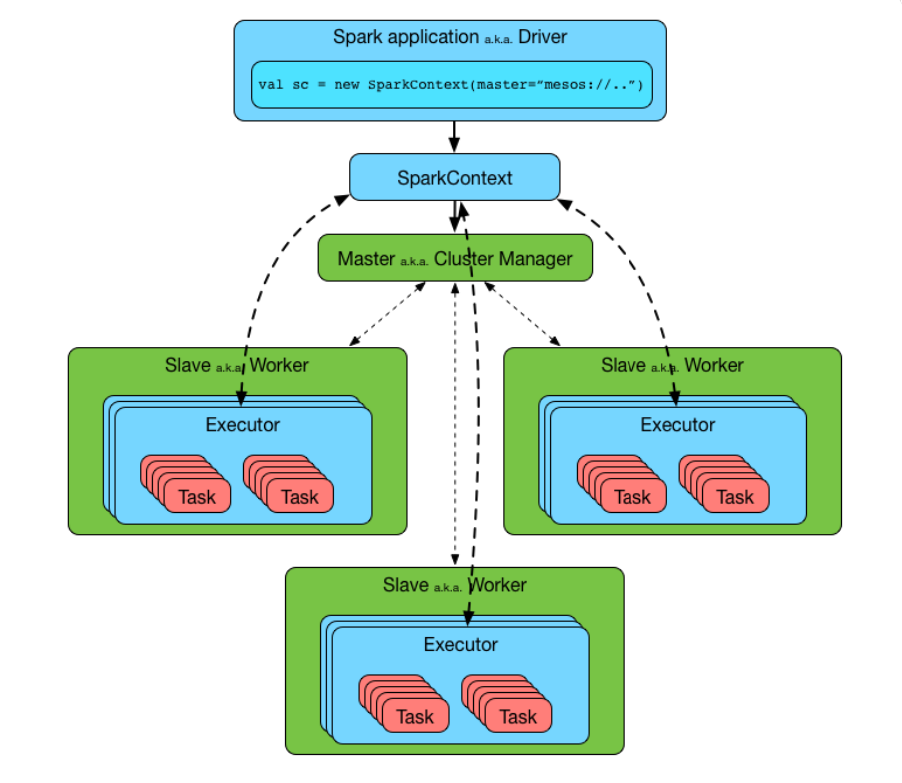
\includegraphics[width=\textwidth]{images/sparkapp2.png}
		\caption{Spark app architecture}
	\end{minipage}
\end{figure}


Spark драйвер отвечает за:
\begin{itemize}
    \item Создание графа вычислений
    \item Оркестрацию вычислений
    \item Управление хранилищем, перемещением данных, доступом к датасетам
    \item Сбор метрик
    \item Обработка ошибок
    \item Запрос ресурсов
\end{itemize}

Spark executor:
\begin{itemize}
    \item Подготовка и исполнение вычислений по задачам
    \item Хранение частей датасетов доступными для нод
    \item Обмен данными с драйвером
    \item Мониторинг
\end{itemize}

Задача состоит из:
\begin{itemize}
    \item Сериализованной функции для вычисления
    \item Список нужных данных
    \item Информация о стадии, к которой принадлежит задача
    \item Настройки среды
\end{itemize}
